
\documentclass[a4paper,10pt]{cpc-hepnp}

%\pdfoutput=1

\usepackage{graphicx}
\usepackage{epstopdf}
\usepackage{subfig}
\usepackage{booktabs}
\usepackage{amssymb,bm,mathrsfs,bbm,amscd}
\usepackage[tbtags]{amsmath}
\usepackage{lastpage}
\usepackage{todonotes}


\begin{document}

\title{electron track direction study in Liquid Scintillator Detector}

\author{%
      Cheng Yaping$^{1}$\email{chengyp@mail.ihep.ac.cn}%
%\quad Li Yufeng$^{2}$\email{liyufeng@mail.ihep.ac.cn}%
%\quad Wen Liangjian$^{2}$
%\quad Lu Jiashu$^{2}$
}
\maketitle
\address{%
$^1$ Institute of High Energy Physics, Chinese
        Academy of Sciences, Beijing 100049, China\\
}


\begin{abstract}
Liquid Scintillator detector features low energy threshold
and good energy resolution. Since scintillation light is isotropic,
we cannot tell the track information from PMT hit pattern.
While Cerenkov light is highly directional, we can derive the track
info of the particles travelling in it under certain circumstances.
The reconstruction performance is discussed if PMT has different TTS and
liquid scintillator has different time components. Also, some potential
usage of lepton track direction reconstruction is also discussed in this manuscript.
\end{abstract}


\begin{keyword}
Liquid Scintillator, Cerenkov light, track direction
\end{keyword}



%%about accelerator neutrino experiment: most of them using water to do flavor discrimination.
%why here using scintillator, need to point out the benefits, that's the usage for it
%%seems section 3.2 is too simply, can it be improved?
%%are there any physics that can use positron direction info when do SN study?
%need to study channel by channel, try to find the possible usage of it.
%%what elements that restrict the track reconstruction performance?
%study whether you can improve it. how about reduce the light yield of the LS, changed it to LAB?

\section{Current efforts towards directionality in neutrino detection}
Neutrino detectors with directionality nature are highly desirable.
Its potential applications are various, including nuclear reactor activity monitoring,
geo-neutrino spatially mapping and background identification.
There are various detection methods used nowadays with direction extraction
ability.

\begin{itemize}
\item Time Projection Chamber
\item Segmented detector
\todo {to be filled \ldots}
\item metal-loaded liquid scintillator
\item Water-based liquid scintillator detector
\end{itemize}

In this manuscript, the track direction reconstruction heavily relied on
detector timing performance. The Flash-ADC readout system combined with
waveform fitting algorithm provide one way to meet the time resolution demand.
The basic principal is to increase the Cerenkov light ratio to about 10\% by selecting early
hits using a time window. Then using a maximum
likelihood method based on photon angular distribution we can reconstruct the
track direction.

\section{General discussion about track direction extraction in LS}

Cerenkov light has unique polarization and directional properties.
Neutrino observatory, such as Super-kamiokande, exploits Cerenkov
light to observe the direction of electrons produced in neutrino
elastic scattering interactions, directly demonstrated that the
sun was a source of neutrinos.
Liquid scintillator neutrino observatory,
such as Daya Bay, mostly exploit scintillation light.
Scintillation light is isotropic, therefore no direction information can be
derived using scintillation light.
\todo {appropriate?}

Firstly, the feasibility to pick up Cerenkov light in a sea of scintillation photons
need to be studied.
All studies are performed under the Geant4 simulation for a large Liquid
scintillator.
The fiducial mass is 20 Kton with LS sphere radius 17.7m.
The PMT photocathode coverage is $\ge$ 75\% and its
quantum efficiency is
$\ge$ 35\%. The attenuation length of the liquid scintillator needs to be $\ge$ 20m at 430 nm.
\todo{more specific}
%\begin{center}
%\includegraphics[width=8.5cm]{eps/detector2.eps}
%\figcaption{\label{LSDetector}   JUNO Liquid Scintillator Detector. }
%\end{center}
%\subsection{principals to separate Cerenkov light and scintillation light}
One possible way to distinguish Cerenkov light and scintillating light is by their hittime
difference\cite{lab2}. We expect PMT detect Cerenkov light earlier than scintillation light.
On the one hand, all Liquid scintillator has fast and slow components. In our
case, the fast and slow time constants are 4.93 and 20.6 ns respectively with
ratio  79.9\% and \%respectively (Table ~\ref{tab1}) .
Therefore, there is a delay of several nanoseconds between the photon emission and the energy deposit.
In the other case, Cerenkov radiation produced from very small displacements by a very large number of electrons
, occurs immediately after the particle has passed and electrons would return to their normal positions
 instantaneously\cite{special_article}.
\begin{center}
\tabcaption{\label{tab1} Time constants of LS }
\footnotesize
\begin{tabular*}{100mm}{@{\extracolsep{\fill}}cccc}
\toprule Particles & Fast(ns)/ratio & Slow(ns)/ratio &Slower(ns)/ratio \\
\hline
$\gamma$,e$^+$,e$^-$&4.93/79.9\%&20.6/17.1\%&190/3.0\% \\
n,p&4.93/65\%&34.0/23.1\%&220/11.9\% \\
$\alpha$&4.93/65\%&35.0/22.8\%&220/12.2\%\\
\bottomrule
\end{tabular*}
\end{center}
On the other hand, Cerenkov radiation spectrum is continuous and it has more
long wavelength
photons ratio than scintillation light Fig.~\ref{figwavelength}. Long
wavelength photon moves faster and has less absorption
and reemission chance in the transportation process in Liquid scintillator.
Both facts makes Cerenkov photon keeps ahead.
\begin{figure}[htbp]
\centering
\begin{minipage}{0.5\textwidth}
\centering
\includegraphics[width=7cm]{eps/wavelength.eps}
\caption{PMT Detected Wavelength Distribution}
\end{minipage}%
\begin{minipage}{0.5\textwidth}
\centering
\includegraphics[width=8cm]{eps/CS_sep.eps}
\caption{Hittime difference}
\end{minipage}
\end{figure}
%\begin{center}
%\includegraphics[width=8.5cm]{eps/wavelength.eps}
%\figcaption{\label{figwavelength}   PMT Detected Wavelength Distribution.}
%\end{center}
%\begin{center}
%\includegraphics[width=8.5cm]{eps/CS_sep.eps}
%\figcaption{\label{figCS_sep}   Hittime difference.}
%\end{center}

Secondly, we need to discuss the impact of multi-scattering on electron tracks.
Physical processes involved include multi-scattering, which changes
particles' momentum direction. A typical track is show in
Fig.~\ref{msc_effect}. The deposited energy by each step is
represented by the marker size and different color indicated the post step
process. The multiple scattering of electrons make the Cerenkov ring fuzzy. In order to
evaluate the intrinsic angular resolution of LS, the deposited energy weighted
angular error is show in Table~\ref{tab2}. Multi-scattering
contributes a lot to electron's drifting away from its original track.
\begin{center}
\includegraphics[width=8.5cm]{eps/msc_effect.eps}
\figcaption{\label{msc_effect} electron track in Liquid Scintillator.}
\end{center}


\begin{center}
\tabcaption{\label{tab2} intrinsic resolution }
\footnotesize
\begin{tabular*}{170mm}{@{\extracolsep{\fill}}ccccccccccc}
\toprule Energy&3&4&5&6&7&8&9&10&11&12\\
\hline
:[$^{\circ}$]&25.38&22.95&22.75&20.88&20.52&18.75&18.17&17.71&17.22&16.2\\
\bottomrule
\end{tabular*}
\end{center}
\todo{necessary?}


\section{electron track direction reconstruction method}
The first step in track direction reconstruction is to get the reconstructed event vertex.
For point-like events, such as e$^+$,e$^-$,$\gamma$, vertex reconstruction was crucial for 
residual time estimation, which is the hit time of the PMT minus the real start time of the event and minus the time of flight for
scintillation photon. The direction reconstruction was relied on the residual time distribution.
For particles generated at detector center, the vertex reconstruction performance from time likehood reconstruction method
was as Fig~\ref{vertexperformance}.
Then, pick up early hits on time of flight subtracted hittime pdf.
For example, if the electron momentum is 3.0 MeV and originated
from the detector center, shooting straightly upwards, then by selecting hits whose hittime is less than 98.8 ns ,almost 50\% of
the hits are generated from Cerenkov photons which contains electron direction information Fig.~\ref{figCS_sep}.
Electron direction determination is by taking the centroid of all vectors pointing from  the vertex to the hits on the
detector Eq.~(\ref{eq1}). Due to scintillation light is isotropic, falsely
picked up scintillation photons will not bias the direction largely.
\begin{center}
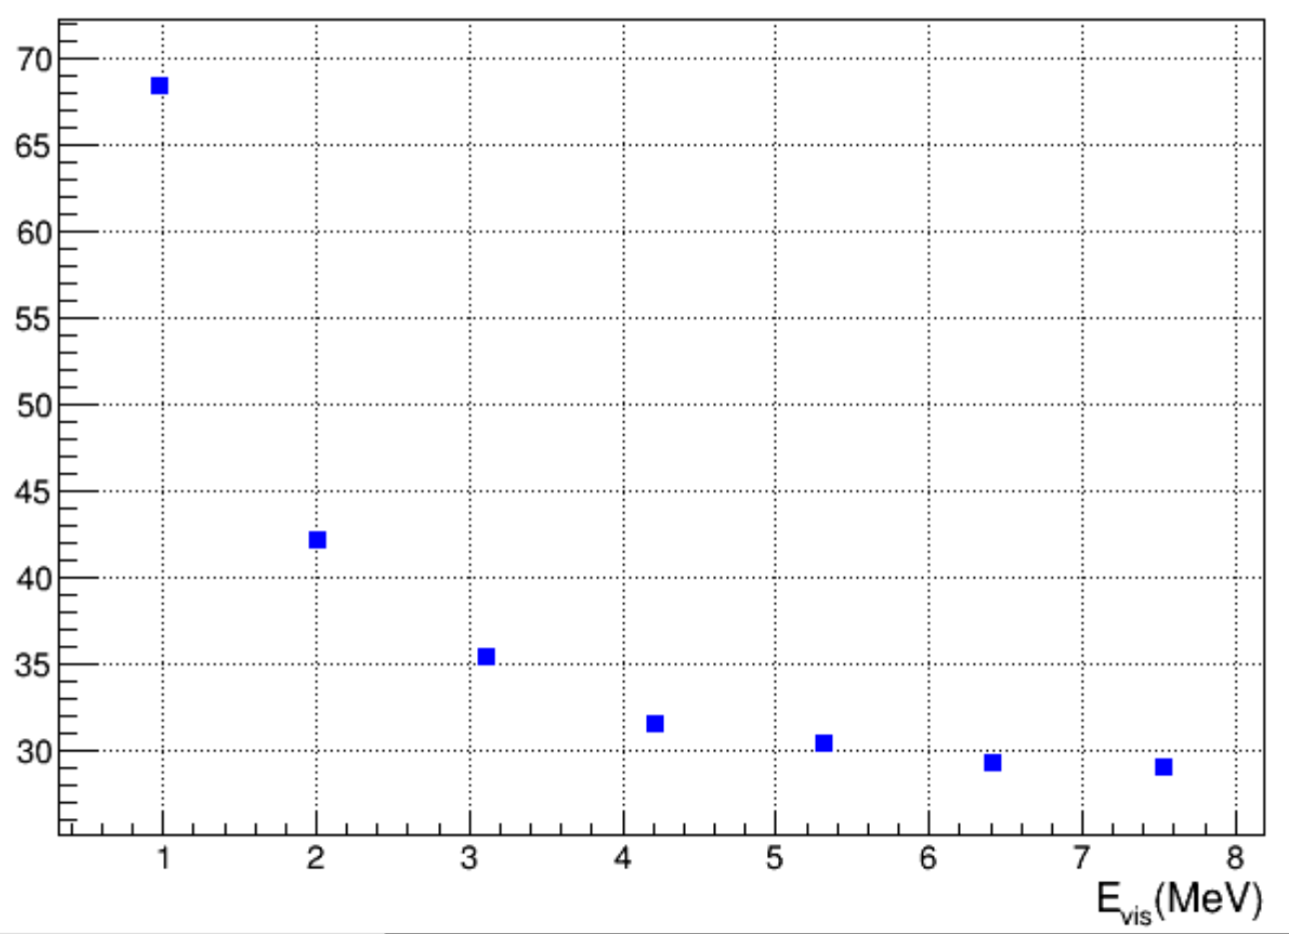
\includegraphics[width=8.5cm]{plots/vertexper}
\figcaption{\label{vertexperformance} vertex reconstruction performance}
\end{center}

\begin{equation}
\label{eq1}
\vec{d_0} = \sum_i{q_i\times{\frac{\vec{P_i}- \vec{O_0}}{\|\vec{P_i}-
\vec{O_0}\|}}}
\end{equation}
here,$\vec{d_0}$is the particle direction,$\vec{O_0}$is the vertex position
derived from vertex reconstruction algorithm.
 $\vec{P_i}$ is the positon and $q_i$ is the charge of the PMT.

\begin{center}
\includegraphics[width=8.5cm]{eps/CS_sep.eps}
\figcaption{\label{figCS_sep}   Hittime difference.}
\end{center}


\section{Likelihood Fit method to derive track direction}
A maximum likelihood method utilizing the Cerenkov and Scintillation light
angular distribution is tested, illuminated by the direction reconstruction
method used by Super-Kamiokande-I \cite{super-k-I}.The likelihood function is
\begin{equation}
\label{eq2}
L(\vec{d_0}) = \sum_i-log((\alpha f(\theta_{dir})+(1-\alpha)g(\theta_{dir}))\times\frac{1.}{CE(\theta_i)}
\end{equation}
where f and g is the PDF function representing opening angle distribution
between the particle track direction and the vector pointing from the vertex to
the center position of fired PMT.$\theta_i$ is the opening angle between the
direction of the vector from the reconstructed vertex to the ith hit PMT
position and PMT  facing  direction. Fig.~\ref{fig_subfig} is the angular distribution
for Cerenkov photon and scintillation photon respectively.
%\end{multicols}
%\ruleup
%\begin{center}
%\includegraphics[width=8.5cm]{eps/angular_pdf_Cerenkov.eps}
%\includegraphics[width=8.5cm]{eps/angular_pdf_scintillation.eps}
%\figcaption{\label{Cerenkov_fraction}   Cerenkov Fraction. }
%\end{center}

\begin{figure*}[htbp]
\centering
\subfloat[Cerenkov]{
\label{fig:improved_subfig_a}
\begin{minipage}[t]{0.5\linewidth}
\centering
\includegraphics[width=8.5cm]{eps/angular_pdf_Cerenkov.eps}
\end{minipage}
}
\subfloat[scintillation]{
\label{fig:improved_subfig_b}
\begin{minipage}[t]{0.5\linewidth}
\centering
\includegraphics[width=8.5cm]{eps/angular_pdf_scintillation.eps}
\end{minipage}
}
\label{fig_subfig}
\caption{angular distribution}
\end{figure*}



%\ruledown
%\begin{multicols}{2}

\subsection{reconstruction performance}
Absolute Cerenkov over scintillation fraction prediction in MC is difficult because of uncertainty in reemission probability.
Fortunately Uncertainty  in  reemission  probability  at  wavelength $>$ 300nm does not significantly affect Cerenkov fraction\cite{DocDB9847}.
The separation of Cerenkov light and scintillation light relies on the recorded hittime from electronics readout system.
Therefore PMT TTS can greatly diminish the power of separation.Besides, the separation power should be energy depended.
For a higher energy,the ratio between direct Cerenkov light and reemitted scintillation light is increasing,as shown in Fig.~\ref{Cerenkov_fraction}.
Here in geant 4 simulation, the input Birk's constant is 6.5$\times10^{-3}g$/$cm^{2}$$/$MeV and the photon yield
is 10400P.e. \/MeV.
\begin{center}
\includegraphics[width=8.5cm]{eps/Cerenkov_fraction.eps}
\figcaption{\label{Cerenkov_fraction}   Cerenkov Fraction. }
\end{center}
\subsubsection{different PMT time performance.}
PMT TTS becomes bottleneck for liquid scintillator detectors' time resolution especially for large area
PMTs with largely varying drifting path. The electronics readout system barely worsen the time resolution
since high speed waveform sampling technology advances a lot in recent years. In the following studies, four sets of
PMT timing performance is considered  (Fig.~\ref{figtts}). One nano seconds TTS could be expected by MCP-PMT,
which can get electron multiplied
millions of times through several millimeter passages.

\begin{center}
\includegraphics[width=8.5cm]{eps/tts.eps}
\figcaption{\label{figtts}  direction reconstruction performance under different PMT tts. }
\end{center}

\subsubsection{energy related track reconstruction performance}
Better track reconstruction performance is ascribed to higher Cerenkov fraction in higher electron kinetic energy,
as shown in Fig.~\ref{Cerenkov_fraction}.In total,10 energy points are simulated.These energy are related to the
energy of prompt signal
from inverse beta decay of reactor antielectron neutrinos. The other two  energy points are provided for future
accelerator neutrino experiments. In  Table~\ref{tab_1sigmaerror}, the 1$\sigma$ error is defined as 68\% reconstructed directions
contained in a cone centered by the true direction within this angle.




\begin{center}
\tabcaption{ \label{tab_1sigmaerror}  reconstruction performance.}
\footnotesize
\begin{tabular*}{190mm}{@{\extracolsep{\fill}}ccccccc}
\toprule kinetic energy/MeV & 1/MeV  & 2/MeV &  3/MeV & 4/MeV &  5/MeV \\
\hline
1 $sigma$ error\hphantom{00} & $95.1^{\circ}$&$78.4^{\circ}$ &$61.1^{\circ}$ &$50.7^{\circ}$&$44.8^{\circ}$\\
\toprule kinetic energy/MeV & 6/MeV & 7/MeV & 8/MeV & 40/MeV & 300/MeV\\
\hline
1 $sigma$ error\hphantom{00} & $39.9^{\circ}$ &$34.1^{\circ}$&$30.6^{\circ}$&$10.2^{\circ}$&$2.4^{\circ}$\\
\bottomrule
\end{tabular*}%
\end{center}






\section{applications}
\subsection{accelerator neutrino experiment}

Accelerator neutrino experiments use $\bar{\nu}_{\mu}$ antineutrinos from $\mu^{+}$ decay  to search $\delta_{CP}$ by detecting
$\bar{\nu}_{\mu}$  to $\bar{\nu}_{e}$  appearance.
By Ref.\cite{angular_corrrelation}, the angular correlation between the incoming antineutrino and
outgoing positron directions can be parameterized  as Eq.~(\ref{eqangular_correlation}).
\begin{eqnarray}
\label{eqangular_correlation}
\begin{aligned}
\left<cos\theta\right>&\approx \frac{\nu^{0}_{e}a^{0}}{3}+\frac{1}{3}\left(3+\frac{4(f+f_{2})g}{f^{2}+3g^{2}}\right)\frac{E_{\nu}}{M}\\
&\approx -0.034\nu^{(0)}_{e} + 2.4\frac{E_{\nu}}{M}
\end{aligned}
\end{eqnarray}
This formula applies to neutrino energy as high as 150MeV, in which case positrons are apparently forward .
For example, 300 MeV electrons can be reconstructed very well as shown in Fig.~\ref{fige300}. Using the
angular correlation,inverse beta decay events can be separated from other reactions or detector backgrounds.
\begin{center}
\includegraphics[width=8.5cm]{eps/e300.eps}
\figcaption{\label{fige300}  direction reconstruction for P=300 MeV electrons. }s
\end{center}
\subsection{supernovae direction determination }
The supernovae is assumed as the explosion in the final stage of the stellar evolution, one of the most violent and spectacular
events in the Universe. A core collapse supernovae (SN) may be not optically visible at all due to dust obscuration or because
some collapsing stars may never blow up into supernovae. However, neutrino signal emerging from the core provides a way to
determine supernovae direction. JUNO detector can detect about 5000 neutrino events from a 10 kpc supernovae.
Neutrino fluxes spectral form are approximately parameterized by Eq.~(\ref{eqnuflux}):Ref\cite{nuflux}.
\begin{eqnarray}
\label{eqnuflux}
\phi(E_{\nu}) &=& N\left(\frac{E_{\nu}}{ \left< E_{\nu}\right>}\right)^{\alpha}exp\left[ -(\alpha+1)\frac{E_{\nu}}{ \left< E_{\nu}\right>}\right]
\end{eqnarray}
In simulation, $\alpha$ was taken to be 3 and mean neutrino energy $\left< E_{\nu}\right>$ was 12.0 MeV.The expected supernova
antielectron neutrino spectra is shown in Fig.~\ref{nuflux_CS}.
\begin{center}
\includegraphics[width=8.5cm]{eps/nuflux_CS.eps}
\figcaption{\label{nuflux_CS}  expected supernova spectra. }
\end{center}

Positron direction information can be reconstructed from above procedures , here 1ns PMT tts is supposed.
Neutrino direction can be calculated on a per event basis using conservation of momentum and energy.
Two difference methods are applied to estimate SN direction. One is the same as \cite{nudir},
SN direction is estimated based on statistically averaged vector pointing from positron vertex to neutron vertex.
SN direction uncertainty is $11.21^{\circ}$. The other method takes the statistically averaged
anti-electron neutrino direction as SN direction, and the SN direction uncertainty is $8.17^{\circ}$.
Thus, it helps supernovae direction determination if additive positron direction information is used.


\section{ Neutrino direction determination via IBD channel}
%\section{Some examples and best-practices}
\label{sec:intro}
In the reaction $\bar{\nu_{e}}+p \rightarrow e^{+}+n$, the
angular distribution of outgoing neutron is strongly forward peaked, with
reference to the injecting neutrino directions. Using the method described in
~\cite{chooz}, direction information can be probed on a  statistical basis.
The vector pointing from the reconstructed positron position to the
reconstructed neutron position was taken as the neutron motion direction.
Figure~\ref{ibd-basicplot} shows the averaged displacement of neutron and
positron from IBD reaction induced by supernova neutrinos and the cosine
projection over the initial neutrino direction. About 5000 IBD events were expected from
supernova 10kpc away. By a simple center mass method denoted as \eqref{cm},
the 68.3\% confidence level error of locating supernova is 13.6 degrees without
vertex smearing. The one standard deviation error is 14.9 when the vertex
reconstruction precision follows $12cm/\sqrt{E}$.
\begin{equation}
\label{cm}
\vec{\nu} = \sum_{i=0}^{N}r_{e^{+}n}
\end{equation}

\begin{figure}[htbp]
\centering % \begin{center}/\end{center} takes some additional vertical space
\includegraphics[width=.45\textwidth]{plots/nerf.pdf}
\hfill
\includegraphics[width=.45\textwidth]{plots/ibd-basicf2.pdf}
% "\includegraphics" is very powerful; the graphicx package is already loaded
\caption{\label{ibd-basicplot} neutron and positron displacement from SN IBD
channel and slightly forward slope towards the neutrino direction.}
\end{figure}
\section{neutrino direction determination via ES channel}
\subsection{basic principals}
Electrons from the neutrino electron elastic scattering (ES) reaction are
strongly forward peaked, electron track direction in LS can be reconstructed
by highly directional Cerenkov light. Assume the refractive index of Liquid Scintillator is 1.46, then the Cerenkov threshold for electron is 0.188 MeV. Thus,plenty of electrons
can have Cerenkov radiation. The challenge is how to pick up more Cerenkov
photons in sea of scintillation photons. One possible way to select more
Cerenkov light is by choosing early hits. Cerenkov light would take the lead in
the race towards PMT photocathode for two reasons. One is Cerenkov light is
produced instantaneously, while scintillation light has slow and fast time
components at nanoseconds time scales. The other is Cerenkov photons have more
long wavelength photons than scintillation photon. For example, the ratio of
photons with wavelength longer than 500nm is 23\% for Cerenkov photon, while
for scintillation the number is about 1\%.
\subsection{reconstruction method}
There are two stages in the reconstruction procedures. The first stage is hit
selection. The aim is to select higher purity of Cerenkov photons. It is
assumed that all scintillation and Cerenkov light is emitted from a single
point. Then residual time is calculated. The point time residual is the
difference between the measured and predicted times of each photon hit.
The predicted time is calculated by using deposited energy vertex from MC truth. The next step
is to select hits in the first 2ns time window in the residual time
distribution plot. After this stage, about ~10\% purity Cerenkov photon purity
is achieved. The next stage is to track direction reconstruction. In total
three methods are tested. The first is center mass method
\eqref{recmethod:1}. The second is orientation matrix method
\eqref{recmethod:2}. The eigenvector with largest eigenvalue represents the
reconstructed track direction. The third method is the Likelihood fitting
method \eqref{recmethod:3}, based on the PMT hit pattern. The predicted hit
pattern took into account the angular distribution PDF of Cerenkov
photons and scintillation photons. The annotations in \eqref{recmethod} are
explained as follows.
Here i,j denotes for three directions. $\alpha$ is the PMT index. $q_{\alpha}$ is the
charge of hits. $\theta_{em}^{\alpha}$  is the photon emission angle. r denotes
the scintillation photon ratio and f,g is the Cerenkov and Scintillation photon
emission angle distribution PDF. Figure~\ref{rec_performance} shows the
reconstruction performance when the particles were at detector center and
shootings towards the positive X axis. The third method gives the best
performance.
\begin{subequations}\label{recmethod}
\begin{align}
\label{recmethod:1}
S_{i} & = \sum_{\alpha=1}^{N}q^{\alpha}x_{i}^{\alpha}
\\
\label{recmethod:2}
(OM)_{ij} & = \sum_{\alpha=1}^{N}q^{\alpha}x_{i}^{\alpha}x_{j}^{\alpha}
\\
\label{recmethod:3}
Lh &= \sum_{i=1}^{N_{pmt}}[(Q^{exp}_{i}-Q^{obs}_{i})+log(\frac{Q^{obs}_{i}}{Q^{exp}_{i}}){\times}Q^{obs}_{i}]
\end{align}
\end{subequations}
The expected charge was calculated as this:
\begin{equation*}
Q^{exp}_{i} = N_{tot}\times[rf(\theta^{em}_{i})+(1-r)g(\theta^{em}_{i})]{\times}h(\theta^{injection}_{i})\times\frac{e^{-\frac{l_i}{L_{att}}}}{l_i^2}
\end{equation*}
%L(\vec{d}) & = -\sum_{\alpha=1}^{N}q_{\alpha}log(rf(\theta_{em}^{\alpha})+(1-r)g(\theta_{em}^{\alpha}))
\begin{figure}[htbp]
\centering % \begin{center}/\end{center} takes some additional vertical space
\includegraphics[width=.85\textwidth]{plots/centerresult}
% "\includegraphics" is very powerful; the graphicx package is already loaded
\caption{\label{rec_performance} direction reconstruction performance.}
\end{figure}
\subsection{absolute photon emission angular distribution PDF construction}
Shape of photon emission angular distribution PDF is derived from MC truth. The
PDF should be the same in LS detector, independent of the event vertex and the
track direction. However, PDF from MC truth was coupled with specific detector
simulation configuration. In my case, my simulation was done under the sniper
framework~\cite{sniper}. The photon angular distribution difference between particles
originated at detector center was caused by different PMT configuration since
PMT was arranged uniformly in the latitude direction.
When the vertexes deviate from detector center, the solid angles of each PMT
and PMT response to photons with different incidence angle, to PMT normal
direction, also contributed to the final angular distribution. Thus, the detector
effects should be removed to get absolute PDF. LS attenuation effect and PMT
angular response was derived from MC truth. The attenuation effect was modeled to
obey the exponential law. By deploying calibration source at certain distance to
PMT and varying the light injection angle, we can probe the PMT angular
response. Figure~\ref{att_angu} shows the fitted attenuation length and PMT
angular response curve to be used to do the detector response correction.
Figure~\ref{xzcomp} shows the Cerenkov and scintillation PDF before and after
detector response correction.
\begin{figure}[htbp]
\centering % \begin{center}/\end{center} takes some additional vertical space
\includegraphics[width=.45\textwidth]{plots/attf.pdf}
\hfill
\includegraphics[width=.45\textwidth]{plots/anguf.pdf}
% "\includegraphics" is very powerful; the graphicx package is already loaded
\caption{\label{att_angu} Attenuation length and angular response.}
\end{figure}
\begin{figure}[htbp]
\centering % \begin{center}/\end{center} takes some additional vertical space
\includegraphics[width=.45\textwidth]{plots/cor_before.pdf}%final1.pdf}
\hfill
\includegraphics[width=.45\textwidth]{plots/cor_after.pdf}%final2.pdf}
% "\includegraphics" is very powerful; the graphicx package is already loaded
\caption{\label{xzcomp} photon emission angular pdf before and after
correction.}
\end{figure}
\subsection{challenges discussion}
\subsubsection{statistical fluctuation}
The basic idea of Likelihood fitting method could be illustrated as the left plot
in Fig~\ref{dis_power}. We discriminate track direction by the region shown in
the plot. For 8 MeV events, in total ~150 hits are selected from reconstruction
stage one, hit selection stage. Some events did not have enough hits in the discrimination power
region. If the Cerenkov bump was not prominent, the scintillation ratio fit
result would fall to 1. In this case, the final direction result was from center mass
method. The ratio fit value falling out to 1 problem  was reproduced by toyMC. If we
enlarged the statistics by 10 times in toyMC, this problem disappeared as shown
in the right plot of Fig~\ref{dis_power}.
\begin{figure}[htbp]
\centering % \begin{center}/\end{center} takes some additional vertical space
\includegraphics[width=.45\textwidth]{plots/dis_power4ratio.pdf}
\includegraphics[width=.45\textwidth]{plots/ratio2.pdf}
% "\includegraphics" is very powerful; the graphicx package is already loaded
\caption{\label{dis_power} statistical fluctuation study.}
\end{figure}
\subsubsection{factors influence residual time distribution}
PMT transit time spread (TTS) could smear the residual time distribution used
in the first stage of direction reconstruction, and makes Cerenkov and
scintillation light separation harder. This effect was taken into
consideration by adding a sampled tts to PMT hittime. The sample was generated
from a Gaussian distribution with mean value 0 and sigma value the assumed
tts. Another significant factor is TOF calculation. At present, it is supposed
that photons travel in straight lines and two effective speed in LS and buffer
was applied(Fig~\ref{caltof_wave_r}). However, this was not true. Light was
refracted on passing through acrylic container and the emission spectrum of PPO
spread from 300 to 650 nm. As shown in Fig~\ref{caltof_wave_r}, when the light path is
longer, the averaged wavelength shift towards longer wavelength.
Fig~\ref{tof_cor} shows the reconstruction performance using single effective
speed and multi effective speed. If we use single effective speed, PMT far
away from the event vertex were more likely to be falsely taken as early hits
in the residual time distribution. This was caused by underestimated TOF of
long light path photons.
\begin{figure}[htbp]
\centering % \begin{center}/\end{center} takes some additional vertical space
%\includegraphics[width=.45\textwidth]{plots/caltof2.pdf}
%\hfill
\includegraphics[width=.45\textwidth]{plots/wave_r.pdf}
% "\includegraphics" is very powerful; the graphicx package is already loaded
\caption{\label{xzcomp} TOF calculation illustration.}
\end{figure}

\begin{figure}[htbp]
\centering % \begin{center}/\end{center} takes some additional vertical space
\includegraphics[width=.45\textwidth]{plots/singlespeedf.pdf}
\hfill
\includegraphics[width=.45\textwidth]{plots/multispeedf.pdf}
% "\includegraphics" is very powerful; the graphicx package is already loaded
\caption{\label{tof_cor} single and multi effective speed comparison.}
\end{figure}
\section{}

The supernova(SN) is assumed as the explosion in the final stage of the
stellar evolution. Determination of a SN explosion direction is essential for
both early stage astronomical observations and optically invisible SN.
Jiangmen Underground Neutrino Observatory(JUNO) has 20 kton liquid
scintillator as target, equipped with more than 18000 PMTs, which provides good
opportunity for SN detection.There are six detection channels in JUNO.
Inverse beta decay(IBD) and neutrino-electron scattering are taken to probe the
supernova direction by utilizing positron and electron track information in
liquid scintillator.

\subsection{SN pointing precision}

If during the lifetime of JUNO a supernova exploded as expected at the center of
    our Galaxy, JUNO would detect 5,000 inverse beta decay
    events, 300 elastic scattering events in the central detector.
%In the JUNO detector, ~300 ES events can be observed.
For SN pointing from ES channel method, the final neutrino direction was the
averaged result from reconstructed electron directions.
The 1$\sigma$ error was defined as the cone angle containing 68.3\%
reconstructed neutrino directions. From Fig~\ref{sn_dir},We can see an improvement from 14.9 degrees to
6.15 degrees from IBD to ES channel in the 1ns PMT tts case. Different distance
supernova and the pointing angular uncertainty was also shown at the right plot
of Fig~\ref{sn_dir}.
%  Expected number of neutrino events in the different interaction channels in
%  SNO+ for a 10kpc supernova, assuming MSW oscillations.(**assuming a 0.2MeV
%  threshold).the number of interactions of each type expected from a 3x1053
%  erg supernova 10kpc from earth
%When a star undergoes a type II supernova explosion, more than 99% of its
%gravitational binding energy is released as neutrinos. This results in more
%neutrinos being produced in the span of a few seconds than are released in
%the rest of the star's life combined. The neutrinos are predicted to be
%evenly distributed among the 3 flavours and to have approximately equal
%numbers of particles and antiparticles. The neutrino flux is so large, in
%fact, that even a supernova at galactic distances should produce a large
%number of events in SNO+. Indeed, neutrinos from supernova 1987A, which
%occurred about 50kpc away from earth in the Large Magellanic Cloud, were
%detected by the KamiokandeII, IMB and Baksan neutrino detectors (11, 8,
%and 5 events, respectively in ~13s). This data has been used for everything
%from testing neutrino oscillation models [1] , to setting limits on
%neutrino mass [2] , to constraining the size of possible compact
%dimensions in the universe [3] . In fact, there is a paper [4] entitled "Yet
%Another Paper on Sn1987a....". If neutrinos from a supernova within our galaxy
%are ever detected, the greater number of observed events would give much
%more information about stellar and neutrino physics.
\begin{figure}[htbp]
\centering % \begin{center}/\end{center} takes some additional vertical space
\includegraphics[width=.43\textwidth]{plots/esresultf.pdf}
\hfill
\includegraphics[width=.55\textwidth]{plots/moredistancesn.pdf}
% "\includegraphics" is very powerful; the graphicx package is already loaded
\caption{\label{sn_dir} SN pointing precision using ES channel.
(left.)reconstructed direction distribution (right.) angular uncertainty and SN
distance}
\end{figure}
%For supernovae neutrinos,the  The positrons could be assumed
%to deposit their energy near the generating vertex. This is reasonable ,for
%example ,in LS, the track length of positron is only about few centimetre.

%For internal references use label-refs: see section~\ref{sec:intro}.
%Bibliographic citations can be done with cite: refs.~\cite{a,b,c}.
%When possible, align equations on the equal sign. The package
%\texttt{amsmath} is already loaded. See \eqref{eq:x}.
%\begin{equation}
%\label{eq:x}
%\begin{split}
%x &= 1 \,,
%\qquad
%y = 2 \,,
%\\
%z &= 3 \,.
%\end{split}
%\end{equation}
%Also, watch out for the punctuation at the end of the equations.
%
%
%
%A similar solution is available for figures via the \texttt{subfigure}
%package (not loaded by default and not shown here).
%All figures and tables should be referenced in the text and should be
%placed at the top of the page where they are first cited or in
%subsequent pages. Positioning them in the source file
%after the paragraph where you first reference them usually yield good
%results. See figure~\ref{fig:i} and table~\ref{tab:i}.
%
%\begin{figure}[htbp]
%\centering % \begin{center}/\end{center} takes some additional vertical space
%\includegraphics[width=.45\textwidth,trim=0 380 0 200,clip]{img1.pdf}
%\hfill
%\includegraphics[width=.45\textwidth]{img2.pdf}
%% "\includegraphics" is very powerful; the graphicx package is already loaded
%\caption{\label{fig:i} Always give a caption.}
%\end{figure}

%\begin{table}[htbp]
%\centering
%\begin{tabular}{|lr|c|}
%\hline
%x&y&x and y\\
%\hline
%a & b & a and b\\
%1 & 2 & 1 and 2\\
%$\alpha$ & $\beta$ & $\alpha$ and $\beta$\\
%\hline
%\end{tabular}
%\caption{\label{tab:i} We prefer to have borders around the tables.}
%\end{table}

%We discourage the use of inline figures (wrapfigure), as they may be
%difficult to position if the page layout changes.
%
%We suggest not to abbreviate: ``section'', ``appendix'', ``figure''
%and ``table'', but ``eq.'' and ``ref.'' are welcome. Also, please do
%not use \texttt{\textbackslash emph} or \texttt{\textbackslash it} for
%latin abbreviaitons: i.e., et al., e.g., vs., etc.
%
%
%
%\section{Sections}
%\subsection{And subsequent}
%\subsubsection{Sub-sections}
%\paragraph{Up to paragraphs.} We find that having more levels usually
%reduces the clarity of the article. Also, we strongly discourage the
%use of non-numbered sections (e.g.~\texttt{\textbackslash
%  subsubsection*}).  Please also see the use of
%``\texttt{\textbackslash texorpdfstring\{\}\{\}}'' to avoid warnings
%from the hyperref package when you have math in the section titles
%
%
%
%\appendix
%\section{Some title}
%Please always give a title also for appendices.
%
%
%
%
%
%\acknowledgments
%
%This is the most common positions for acknowledgments. A macro is
%available to maintain the same layout and spelling of the heading.
%
%\paragraph{Note added.} This is also a good position for notes added
%after the paper has been written.
%
%



% The bibliography will probably be heavily edited during typesetting.
% We'll parse it and, using the arxiv number or the journal data, will
% query inspire, trying to verify the data (this will probalby spot
% eventual typos) and retrive the document DOI and eventual errata.
% We however suggest to always provide author, title and journal data:
% in short all the informations that clearly identify a document.





\vspace{-1mm}
\centerline{\rule{80mm}{0.1pt}}
\vspace{2mm}




\begin{thebibliography}{90}

\vspace{3mm}

\bibitem{chooz}
M.Apollonio{\it et al.}  \emph{Determination of neutrino incoming
direction in the CHOOZ experiment and its application to
supernova explosion location by scintillator detectors
}, \emph{Phys.\ Rev.\ D } {\bf 61} (1999) 012001.

\bibitem{sniper}
http://juno.ihep.ac.cn/mediawiki/index.php/Main\_Page
\bibitem{b}
Author, \emph{Title},
arxiv:1234.5678.

\bibitem{c}
Author, \emph{Title},
Publisher (year).




\bibitem{lab1} http://highenergy.phys.ttu.edu/dream/resources\\
/publications/550\_185.pdf
\bibitem{lab2} http://arxiv.org/pdf/1307.5813.pdf
\bibitem{lab3}  arXiv:1409.5864
\bibitem{special_article} Cerenkov raditon and its applications\\
 J V Helley
\bibitem{nuflux} L. Huedepohl, B. Muller, H. T. Janka, A. Marek,\\
 and G. G. Raffelt, Phys. Rev. Lett. 104, 251101 (2010), 0912.0260.
\bibitem{push_and_pull} http://kamland.lbl.gov/Dissertations\\
/LindleyWinslow-DoctorThesis.pdf
\bibitem{DocDB9847} http://dayabay.ihep.ac.cn/DocDB/0098/009847\\
/002/cfrac\_etw.pdf
\bibitem{nudir} Phys.Rev.D 61 (1999) 012001
\bibitem{angular_corrrelation} http://arxiv.org/pdf/hep-ph/\\
9903554.pdf
\bibitem{PhysRevD.61.012001}M. Apollonio \emph{et al.} Phys. Rev. D \textbf{61}, 012001,1999
\bibitem{PhysRevD.73.112001}J. Hosaka\emph{et al.} Phys. Rev. D \textbf{73}, 112001,2006
\end{thebibliography}


\clearpage

\end{document}

